\section{The ATLAS Detector}
\label{sec:atlas}

In this section we will extend our focus to the ATLAS detector, the general purpose
particle detector located at Point 1 of the LHC ring (see Figure~\ref{fig:p1}).
Roughly cylindrical in shape, coaxial with the beam-pipe,
the ATLAS detector is 44\,m long and 25\,m tall.
It is by far the largest such detector ever built and,
generally, is the largest and most complex device ever constructed.
Being general purpose in scope, the ATLAS detector is hermetic and has
nearly $4\pi$ radians of solid angle coverage around the $pp$ collision
point. 
Such detectors are commonly designed to have various subsystems --- \textit{subdetectors} ---
which are designed for the identification of specific types of particles
and interactions.
They tend to be layered about the interaction point and cylindrically symmetric
since the $pp$ interactions taking place within the detector have no preferred
direction in the plane transverse to the direction in which the proton beams
are travelling.
A view of the ATLAS detector and its subdetectors is provided by Figure~\ref{fig:atlas_cutaway}.
In the following we will briefly describe each subsystem in turn, describing
first the detectors located nearer to the $pp$ collision and proceeding outwards.

\subsection{The ATLAS Coordinate System}
\label{sec:atlas_coordinate_system}

The ATLAS detector uses a right-handed coordinate system with the origin located at
the geometric center of the detector.
The $x$-axis points to the center of the LHC ring, the $y$-axis points upwards
and away from the center of the Earth, and the $z$-axis is along the beam-pipe.
The side associated with positive (negative) $z$
is referred to as the `A' (`C') side of the detector.\footnote{`A' for `airport',
since this is the side pointing towards Geneva International Airport, and
`C' for either `Crozet' or `Charly's', depending on who you ask, since this is the side
pointing towards the town of Crozet and/or Charly's Pub in the town of Saint-Genis-Pouilly.}
Due to its cylindrical symmetry, ATLAS also uses the cylindrical coordinates, $(r,\phi, z)$,
with $\phi$ the azimuthal angle about the $z$-axis and having $\phi = 0$ along the positive $x$-axis.
The spherical polar angle, $\theta$, is defined with respect to the $z$-axis, having
$\theta = 0$ parallel to the beam-pipe and $\theta = \pi/2$ in the $xy$-plane transverse
to the beam-pipe.
The pseudorapidity, $\eta$, is commonly used when describing systems of particles or locations within
the detector and is defined as $\eta = - \ln \left[ \tan \left( \theta / 2 \right) \right ]$.
The relationship between pseudorapidity and polar angle is illustrated in Figure~\ref{fig:eta_desc}.
Large (small) values of $\eta$ correspond to the \textit{forward} (\textit{central}) region of the detector.
The rapidity, $y$, is related to $\eta$ and is defined as $y = \frac{1}{2} \ln \left[ (E+p_z) / (E-p_z) \right]$.
The pseudorapidity of a particle traversing the detector is equal to its rapidity if
the particle is massless or ultra-relativistic; otherwise, they are different.
The comparison between a particle's pseudorapidity and rapidity is illustrated in
Figure~\ref{fig:eta_desc}.
The coordinates used to describe systems of particles are typically described by their
four-momenta: $(p_x, p_y, p_z)$ or, equivalently, $(\pT, \eta, \phi)$.
A distance metric commonly used to describe the distance between two systems of particles
in the detector is $\Delta R = \sqrt{ (\Delta \eta)^2 + (\Delta \phi)^2 }$. The
$\Delta R$ quantity using $y$ instead of $\eta$ is also sometimes used and will be
indicated by $\Delta R_y$.

\begin{figure}[!htb]
    \begin{center}
        \raisebox{1.5cm}{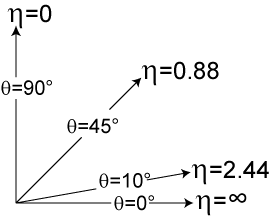
\includegraphics[width=0.35\textwidth]{figures/chapter2/eta_vs_polar}}
        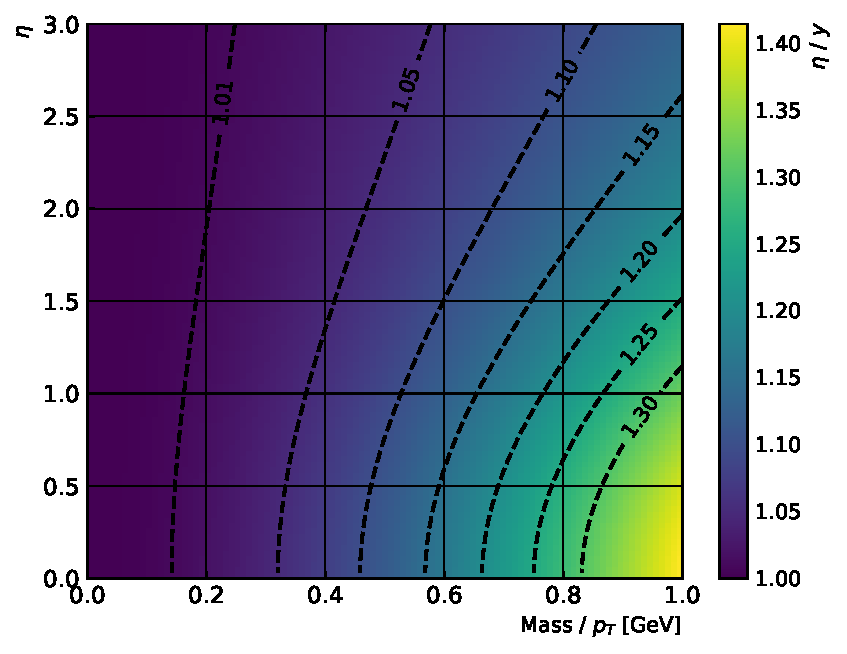
\includegraphics[width=0.55\textwidth]{figures/chapter2/eta_vs_rap}
        \caption{
            \textbf{\textit{Left}}: Illustration of the relationship between the pseudorapidity, $\eta$,
                and polar angle, $\theta$, defined as the angle with respect to the beam-axis ($z$-axis).
            \textbf{\textit{Right}}: Distribution of the ratio of a particle's pseudorapidity to its rapidity, $\eta$/$y$,
                as a function of its pseudorapidity ($y$-axis) and the ratio of its mass to its transverse momentum, \pT~($x$-axis).
        }
        \label{fig:eta_desc}
    \end{center}
\end{figure}


\begin{figure}[!htb]
    \begin{center}
        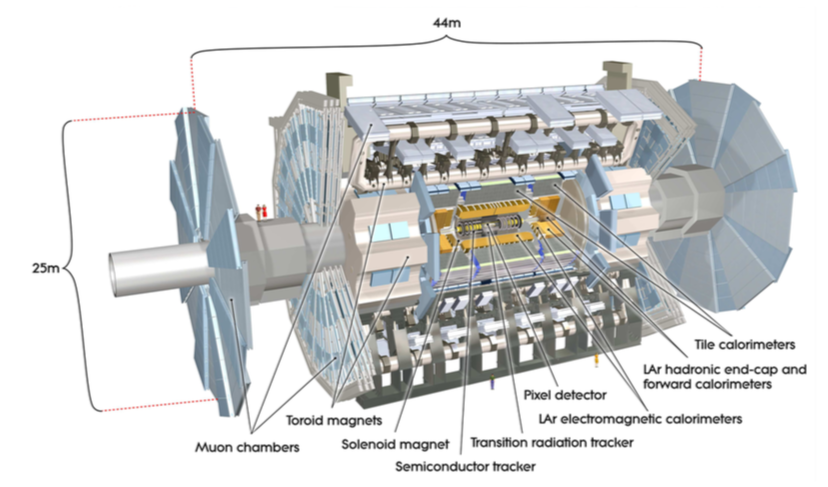
\includegraphics[width=0.95\textwidth]{figures/chapter2/atlas_cutaway}
        \caption{
            Cut-away view of the ATLAS detector with sub-systems indicated.
            Shown for comparison are figures of average-height humans standing
            at the feet of the detector and standing on the forward shielding
            between the big wheels of the forward muon system.
            Figure taken from Ref.~\cite{ATLASCollab}.
        }
        \label{fig:atlas_cutaway}
    \end{center}
\end{figure}


\begin{figure}[!htb]
    \begin{center}
        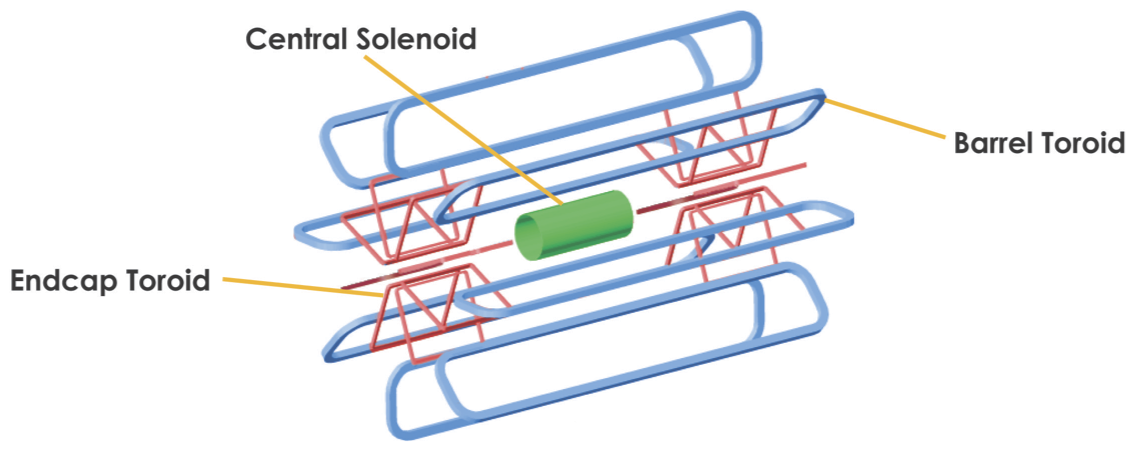
\includegraphics[width=0.95\textwidth]{figures/chapter2/atlas_magnet_system}
        \caption{
            A view of the ATLAS magnet system. Shown are the 2\,T solenoid magnet
            in green, the barrel toroid system in blue, and endcap toroid magnets
            in red.
            Figure taken from Ref.~\cite{CERN-LHCC-97-018}.
        }
        \label{fig:atlas_magnet_system}
    \end{center}
\end{figure}

%%%%%%%%%%%%%%%%%%%%%%%%%%%%%%%%%%%%%%%%%%%%%%%%%%%%%%%%%%%%%%%%%%%%%
%%%%%%%%%%%%%%%%%%%%%%%%%%%%%%%%%%%%%%%%%%%%%%%%%%%%%%%%%%%%%%%%%%%%%
%
% INNER DETECTOR
%
%%%%%%%%%%%%%%%%%%%%%%%%%%%%%%%%%%%%%%%%%%%%%%%%%%%%%%%%%%%%%%%%%%%%%
%%%%%%%%%%%%%%%%%%%%%%%%%%%%%%%%%%%%%%%%%%%%%%%%%%%%%%%%%%%%%%%%%%%%%
\subsection{The Inner Detector}
\label{sec:inner_detector}

The innermost subdetector of ATLAS is the Inner Detector (ID)~\cite{Haywood:331064}.
The ID covers the region $\lvert \eta \rvert < 2.5$ and is composed, in order
of increasing radial distance from the beam-pipe, of the silicon pixel detector,
the silicon-strip semiconductor tracker (SCT), and the transition radiation tracker (TRT).
These detectors enable the reconstruction of the tracks associated with
the $\mathcal{O}(1000)$ charged particles emerging from each $pp$ bunch collision occurring
every 25\,ns.
An illustration of the ID and its subdetectors is shown in Figure~\ref{fig:atlas_inner_detector}.
Additional, more detailed views of the barrel and endcap sections of the ID are shown in Figure~\ref{fig:atlas_ID_exploded}.
Figure~\ref{fig:atlas_ID_plan_view} shows further information about the physical locations in $r$, $z$, and $\eta$
of each of the components that make up the ID.
The ID is situated inside of the central solenoid, indicated in Figure~\ref{fig:atlas_magnet_system},
which provides an axial 2\,T magnetic field and extends over a length of 5.3\,m with a diameter of 2.5\,m.
The bending of charged particles in the $xy$-plane due to the presence of the solenoidal
field allows for their momenta to be measured using the curvature of their reconstructed tracks.

\begin{figure}[!htb]
    \begin{center}
        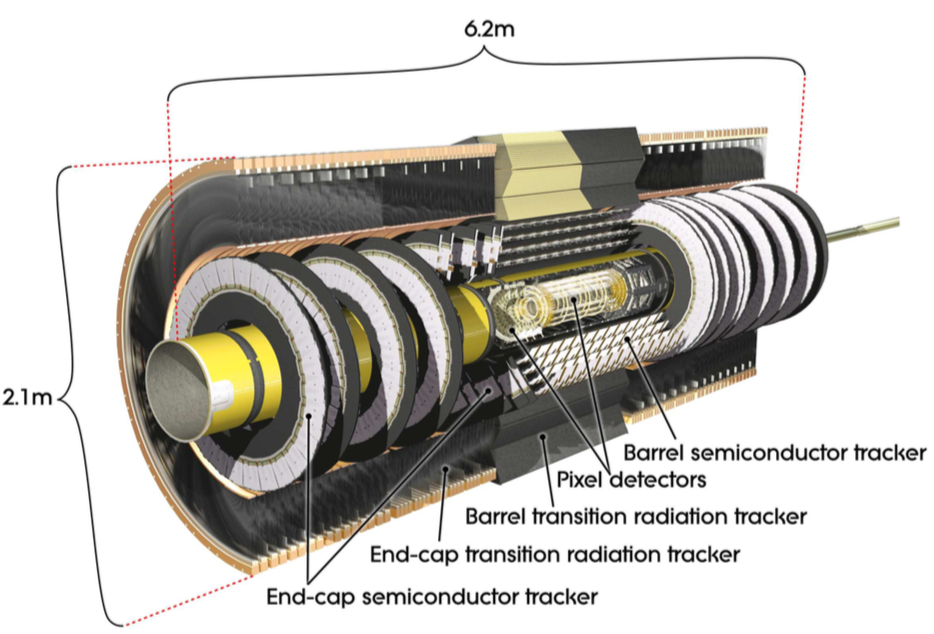
\includegraphics[width=0.75\textwidth]{figures/chapter2/inner_detector/atlas_inner_detector}
        \caption{
            Cross-sectional view of the ATLAS inner detector. Shown are the barrel
            and end-cap portions of the pixel, SCT, and TRT detectors.
            Figure taken from Ref.~\cite{ATLASCollab}.
        }
        \label{fig:atlas_inner_detector}
    \end{center}
\end{figure}

\begin{figure}[!htb]
    \begin{center}
        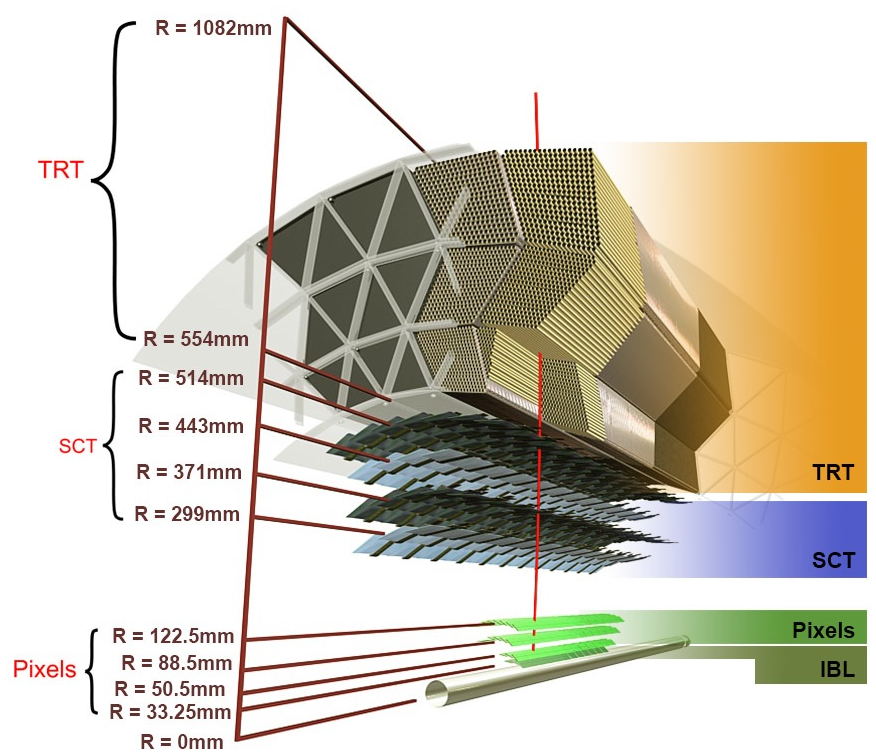
\includegraphics[width=0.7\textwidth]{figures/chapter2/inner_detector/atlas_ID_barrel_exploded}
        \raisebox{1.4cm}{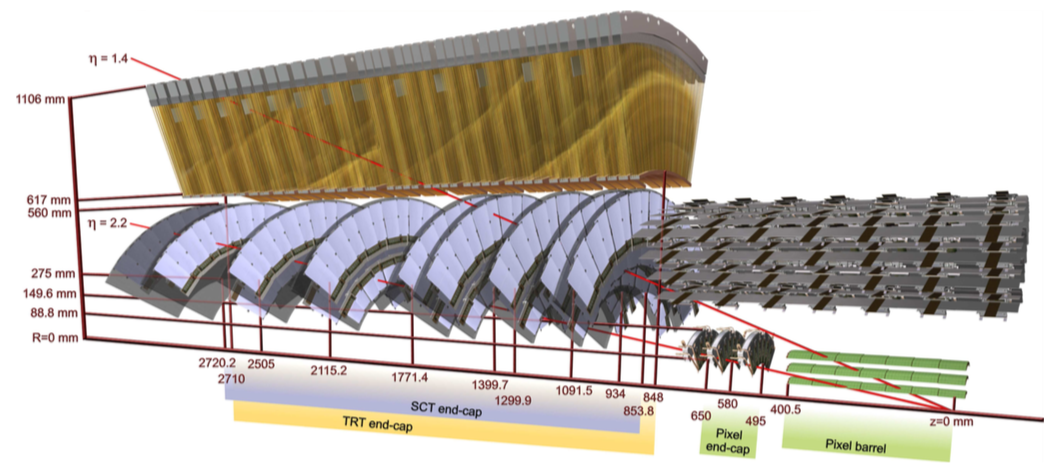
\includegraphics[width=0.95\textwidth]{figures/chapter2/inner_detector/endcap_ID_exploded}}
        \caption{
            Cut-away views of the barrel (\textit{\textbf{top}}) and end-cap (\textit{\textbf{bottom}}) portions
            of the ATLAS inner detector, with each of the three subdetectors indicated along with their
            envelopes in $r$ and in $z$.
            Figure taken from Ref.~\cite{ATLASCollab}.
        }
        \label{fig:atlas_ID_exploded}
    \end{center}
\end{figure}

\begin{figure}[!htb]
    \begin{center}
        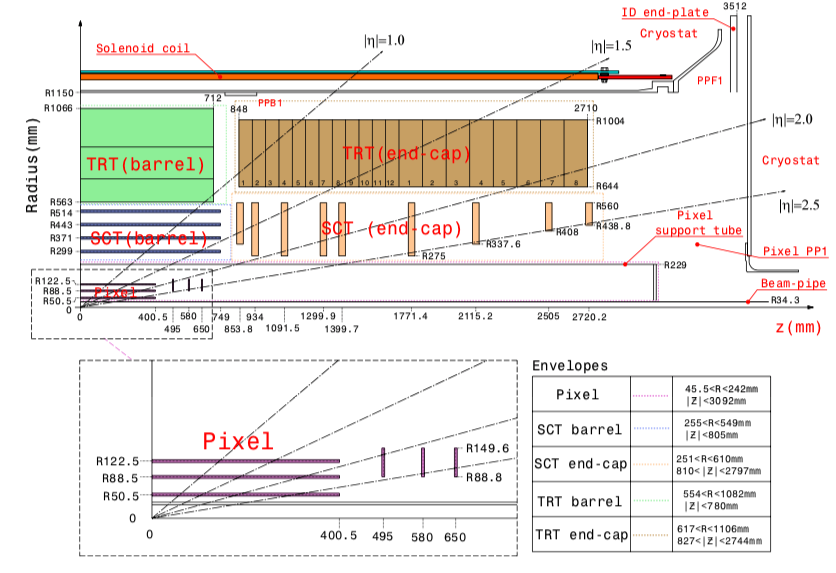
\includegraphics[width=0.9\textwidth]{figures/chapter2/inner_detector/atlas_ID_plan_view}
        \caption{
            Detailed drawing of the locations of the subsystems that make up the ATLAS ID.
            Positions in $r$, $z$, and $\eta$ are shown.
            Figure taken from Ref.~\cite{ATLASCollab}.
        }
        \label{fig:atlas_ID_plan_view}
    \end{center}
\end{figure}

\subsubsection{The Pixel Detector and IBL}
\label{sec:id_pixel}

The pixel detector is the innermost subdetector of the ID, situated very near to and surrounding
the beam-pipe.
It is composed of three separate sections: a barrel section and two end-cap sections.
The barrel section  of the pixel detector has a cylindrical geometry and the end-cap sections
are disks centered on the beam-pipe.
The barrel section has four layers, each with increasing radius, and there are three disks in each
of the end-caps. This ID geometry, shown in Figure~\ref{fig:atlas_ID_exploded}, covers
the region $\lvert \eta \rvert < 2.5$.

The pixel detector, being so near the $pp$ collisions, is subject to the highest particle
fluxes of any other subsystem.
As a result, it is built to have very fine granularity: its sensing elements consist of
$250$\,\micron~thick detectors housing pixels of reverse-biased n-type silicon semiconductor material,
each having a nominal size of $50\times400\,\micron^2$.
In total, there are roughly 80 million channels read out from the pixel detector alone.
This allows for the pixel detector's fine spatial hit resolution of $10\,\micron$ in
$(r-\phi)$ and $115\,\micron$ along $z$.

The innermost layer of the pixel detector's barrel section is referred to as the
\textit{Insertable B-Layer} (IBL), and was installed at the beginning of the Run 2
data-taking period~\cite{Capeans:1291633}.
It corresponds, essentially, to the instrumentation of the ATLAS beam-pipe, as seen in Figure~\ref{fig:pixel_detector_trans},
and is located at a radial distance of 3.3\,cm.
It alone accounts for 8 million readout channels of
the pixel detector --- resulting in an ultra precise spatial hit resolution of $8\,\micron$ in $(r-\phi)$ and
$40\,\micron$ along $z$.
Beyond improving the overall measurements and reconstruction of charged particle tracks,
the IBL was installed in order to improve the performance of secondary vertex
reconstruction --- an essential ingredient to the algorithms associated with
the reconstruction and identification of jets originating from the decays
of $b$-hadrons whose decays occur at radial distances frequently beyond that
of the IBL, as illustrated in Figure~\ref{fig:bhadron_decay_length}..

\begin{figure}[!htb]
    \begin{center}
        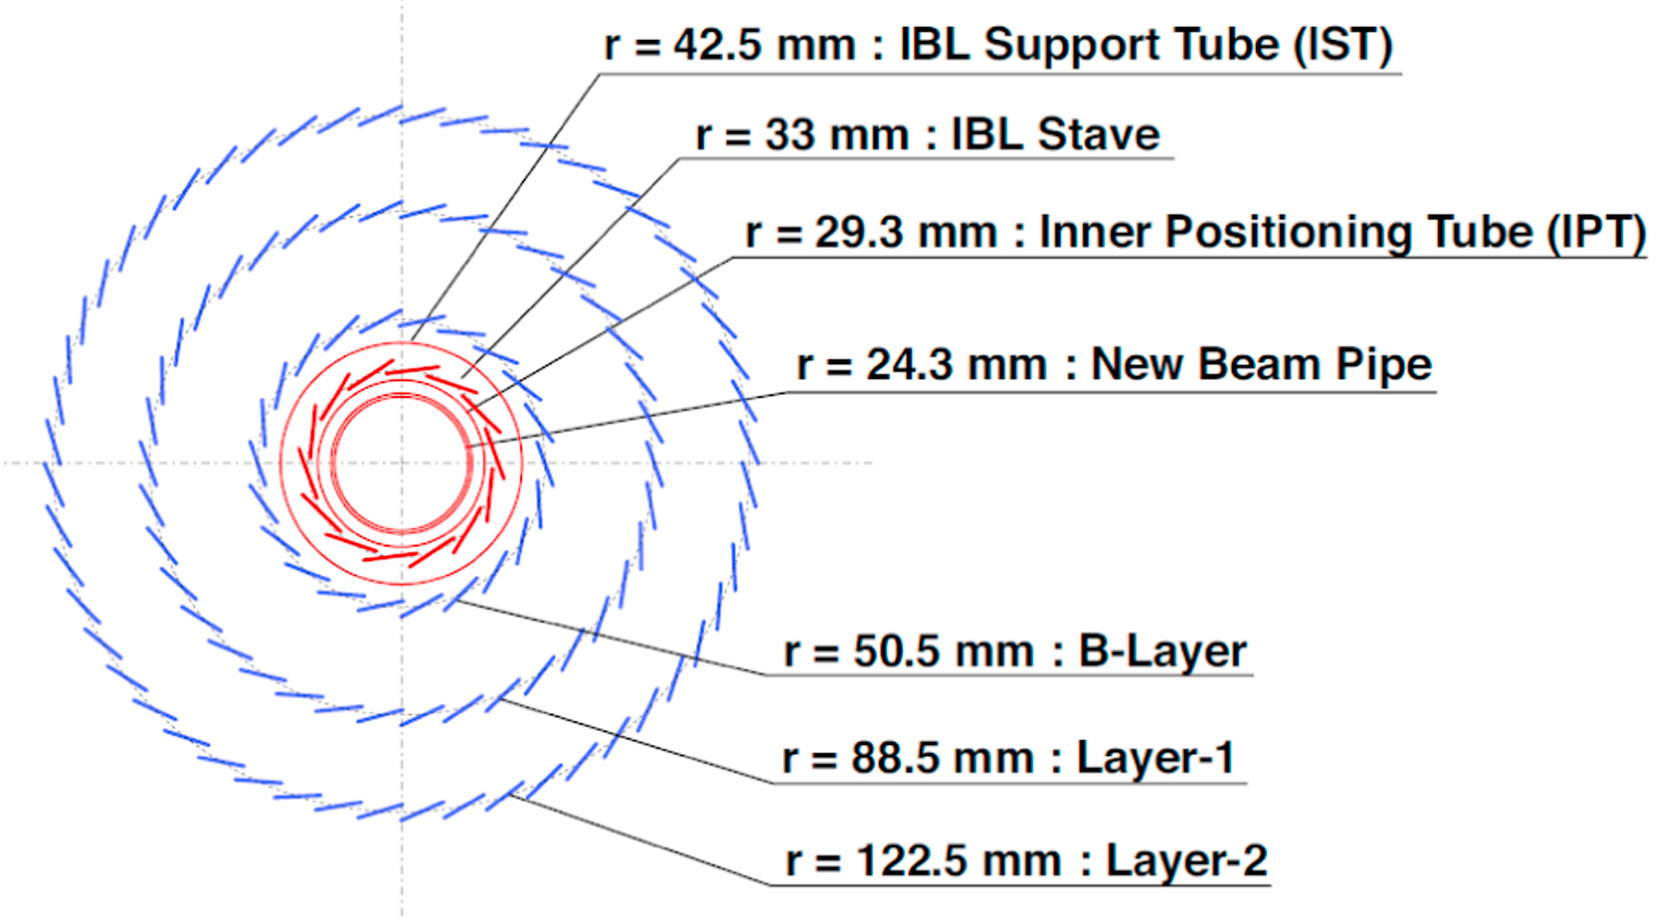
\includegraphics[width=0.8\textwidth]{figures/chapter2/inner_detector/pixel_detector_trans}
        \caption{
            Transverse view of the barrel section of the pixel detector, showing
            the innermost layer, the Insertable B-Layer (IBL), and its support structure (red) as well as the
            three surrounding layers (blue). Figure taken from Ref.~\cite{Backhaus:2016ctq}.
        }
        \label{fig:pixel_detector_trans}
    \end{center}
\end{figure}

\subsubsection{The Semiconductor Tracker}
\label{sec:id_sct}

The semiconductor tracker (SCT), like the pixel detector, uses silicon semiconductor-based sensing
elements.
It surrounds the pixel detector, as illustrated in Figure~\ref{fig:atlas_ID_exploded},
and has similar barrel and end-cap geometries.
The barrel section of the SCT is composed of 4 cylindrical layers and the end-caps consist
of 9 disks.
The silicon sensing elements are in a strip-like geometry with
$80\,\micron$ strip pitch.
The strips in the barrel section run parallel to the beam-pipe and those in the
end-caps are perpendicular, extending along the radial direction.\footnote{
The SCT layers in both the barrel and end-cap sections additionally contain small-angle (40\,mrad) stereo strips (c.f. Figure~\ref{fig:mm_stereo}) to allow for measurement of both
$(r-\phi)$ and $z$ information.}
The spatial hit resolution of the SCT is $17\,\micron$ in $(r-\phi)$ and $580\,\micron$
along $z$.

\subsubsection{The Transition Radiation Tracker}
\label{sec:trt}

The outermost layer of the ATLAS ID, surrounding the SCT, is the transition
radiation tracker (TRT).
The TRT is a tracking volume designed around the proportional drift tube concept
and is composed of polyimide drift tubes (straws) that are 4\,mm in diameter.
The barrel section of the TRT contains up to 73 layers of 144\,cm-long straws aligned parallel to the
beam-pipe while the end-cap section has 160 straw planes composed of 37\,cm long straws arranged radially
into wheels (see Figure~\ref{fig:atlas_ID_exploded}).
Each straw of the TRT has a 31\,\micron~-width gold-coated wire at its center which acts as anode
and is grounded, while the inner walls of each straw are kept at a potential of
approximately $-1.5$\,kV.
A track hit in a given straw is the result of the 70\% Xe -- 27\% CO$_2$ -- 3\% O$_2$ gas mixture contained
in the straw volume being ionised and the resulting electrons (ions) drifting to
the center wire (inner wall) of the straw. The induced current from the drifting
charge is converted to an electrical signal and read out.

On average, a single charged-particle track leaves 36 hits in the TRT.
The TRT only provides $(r-\phi)$ information (no $z$ information),
for which it has a per-straw hit resolution of $130\,\micron$.
The relatively poor hit resolution, when compared to the silicon based
tracking detectors, is compensated by the large number of hits per track which
lead to very long measured track lengths as compared to the pixel and SCT detectors.
Additionally, the straws are embedded in and individually separated by
a polypropylene fiber which induces transition-radiation photons to be produced.
The amount and pattern of transition radiation depends on the mass of the passing
particle: the passage of an electron will produce significantly more transition radiation
than heavier charged particles, such as the copiously-produced pion.
Information provided by the TRT therefore provides additional discrimination
power between electrons and pions and enhances the performance of ATLAS' electron identification algorithms
that primarily depend on information coming from the calorimeter systems (Section~\ref{sec:calo_em}).


%%%%%%%%%%%%%%%%%%%%%%%%%%%%%%%%%%%%%%%%%%%%%%%%%%%%%%%%%%%%%%%%%%%%%
%%%%%%%%%%%%%%%%%%%%%%%%%%%%%%%%%%%%%%%%%%%%%%%%%%%%%%%%%%%%%%%%%%%%%
%
% CALORIMETERS
%
%%%%%%%%%%%%%%%%%%%%%%%%%%%%%%%%%%%%%%%%%%%%%%%%%%%%%%%%%%%%%%%%%%%%%
%%%%%%%%%%%%%%%%%%%%%%%%%%%%%%%%%%%%%%%%%%%%%%%%%%%%%%%%%%%%%%%%%%%%%
\subsection{Calorimeter Systems}
\label{sec:calorimeters}

The ATLAS calorimeter systems are situated outside of the ID and central solenoid and
are tasked with the measurement and containment of showers from electrically charged and neutral particles.
A view of the calorimeter systems is provided by Figure~\ref{fig:atlas_calorimeters_cutaway}.
Broadly speaking, there are two types of calorimeters based on their purpose:
electromagnetic and hadronic calorimeters.
The electromagnetic calorimeter system has $\eta$ coverage that matches the inner-detector
and is optimized for precision measurements of electrons and photons.
The hadronic calorimeter system has readout cells that are generally of
coarser granularity as compared to the electromagnetic calorimeter and
is designed to meet the requirements for jet and missing transverse momentum
measurements.
Besides classification by physics purpose, the calorimeter system can also
be broken into two classes based on detector technology: either based
on gaps of cooled liquid-argon~\cite{CERN-LHCC-96-041} or on scintillating tiles as the active media~\cite{CERN-LHCC-96-042}.

\begin{figure}[!htb]
    \begin{center}
        \includegraphics[width=0.9\textwidth]{figures/chapter2/calorimeters/atlas_calorimeter_cutaway}
        \caption{
            Cut-away view of the ATLAS calorimeter system, with liquid-argon and scintillating-tile
            subsystems indicated.
            Figure taken from Ref.~\cite{ATLASCollab}.
        }
        \label{fig:atlas_calorimeters_cutaway}
    \end{center}
\end{figure}

\subsubsection{Electromagnetic Calorimeter}
\label{sec:calo_em}

The electromagnetic (EM) calorimeter is a high-granularity lead/liquid-argon (LAr)
sampling calorimeter situated outside of the ID and sharing the
same cryostat as the central solenoid.
It consists of barrel and end-cap sections that cover the entire
range within $\lvert \eta \rvert < 3.2$ and is illustrated in Figure~\ref{fig:atlas_calorimeters_cutaway}.
The structures of the electromagnetic barrel and end-cap calorimeters
are shown in Figure~\ref{fig:em_calo_section}.
The EM calorimeter is designed in an accordion type structure to provide full coverage
in $\phi$.
The cooled LAr fills the gaps between layers of the
accordion structure.
Passing particles from the interaction point undergo scattering and bremsstrahlung processes as they pass through
the lead absorbers. The resulting electrons and photons ionise the LAr, producing
drift electrons and ions whose signals are read out by the interleaved readout
electrodes. The 2.1\,mm drift gap has an operating voltage of $\approx 2$\,kV.
The electromagnetic calorimeter is $>22$ radiation lengths ($X_0$), ensuring
that the majority of electrons and photons are completely contained within the EM calorimeter.
The majority of the EM energy, amounting to approximately 16\,$X_0$, is contained
within the second sampling layer (see Figure~\ref{fig:em_calo_section}).
The fine granularity of the readout, indicated in Figure~\ref{fig:em_calo_section},
was designed with the ability to distinguish individual photons arising from $\pi^0 \rightarrow \gamma \gamma$
decays. The ability to distinguish photons pairs so precisely is also important for the
main Higgs boson decay channel used for its discovery, $h \rightarrow \gamma \gamma$.

In the region $\lvert \eta \rvert < 1.8$, a so-called \textit{presampler} detector is used to correct
for the energy lost by electrons and photons due to material interactions occurring
upstream of the EM calorimeter.
It is a single LAr layer, with width 1.1\,cm (0.5\,cm) in the barrel (end-cap).

\begin{figure}[!htb]
    \begin{center}
        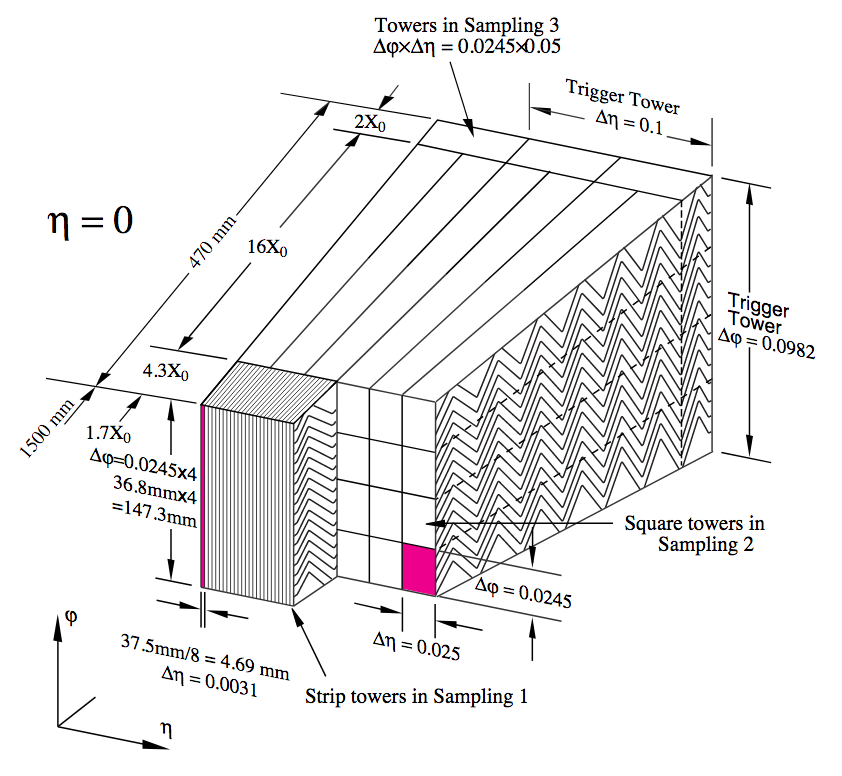
\includegraphics[width=0.6\textwidth]{figures/chapter2/calorimeters/atlas_em_calo_barrel}
        \raisebox{1.5cm}{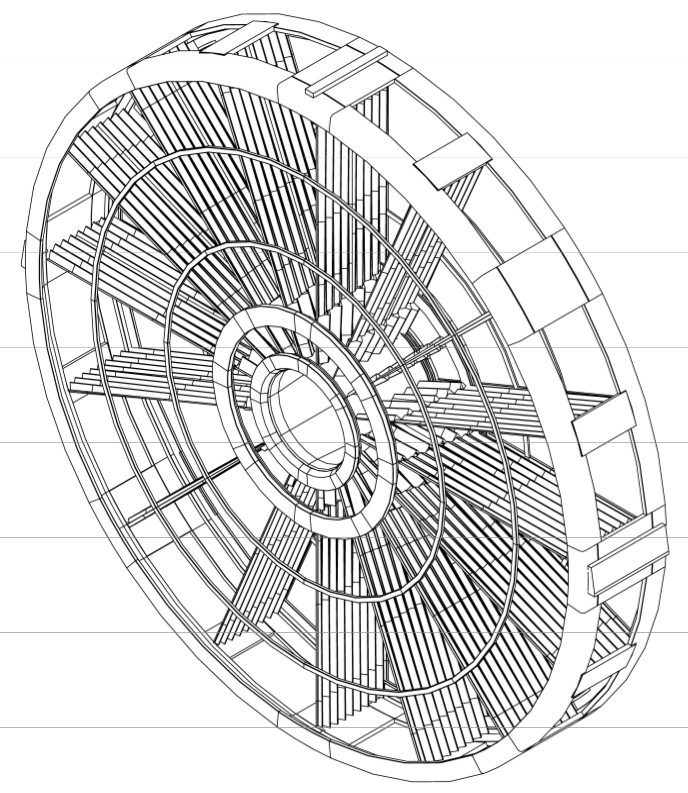
\includegraphics[width=0.3\textwidth]{figures/chapter2/calorimeters/atlas_em_calo_endcap}}
        \caption{
            Figures taken from Ref.~\cite{CERN-LHCC-96-041}.
            \textbf{\textit{Left}}: Cut-away view of the barrel electromagnetic calorimeter and its accordion
                structure. Indicated are
                the geometry and absorption properties of the three sampling layers.
                Also indicated is the granularity of the electrode readout in $\Delta \phi \times \Delta \eta$
                in each layer.
            \textbf{\textit{Right}}: Diagram of the electromagnetic end-cap calorimeter accordion wheel structure
                (only a sub-set of the accordion structure is shown).
        }
        \label{fig:em_calo_section}
    \end{center}
\end{figure}

\FloatBarrier
\subsubsection{Hadronic Calorimeter}
\label{sec:calo_had}

The barrel section of the hadronic calorimeter is composed of a
lead/scintillating-tile type detector whereas the end-cap hadronic
calorimeter is based on copper/LAr-based technology.

The lead/scintillating-tile calorimeter (the `tile calorimeter') is located just beyond
the EM calorimeter.
It is composed of a barrel section, covering $\lvert \eta \rvert < 1.0$,
and two extended barrels that cover $0.8 < \lvert \eta \rvert < 1.7$ (see Figure~\ref{fig:atlas_calorimeters_cutaway}).
It is a sampling calorimeter using steel as the passive absorber and scintillating
plastic tiles as the active media.
The tile calorimeter is composed of modules in which the scintillating
tiles are situated in $(r-\phi)$ within the steel absorbers, as shown in Figure~\ref{fig:tile_calo}.
The detector is segmented radially into three layers and the readout of the
scintillation light, using wavelength-shifting fibers that are fed into photomultiplier tubes (PMT)
situated along the outer radii, is organized in a projective
geometry, also illustrated in Figure~\ref{fig:tile_calo}.
In the barrel (extended barrel) section, most of the hadronic energy is captured by the first (last) two
layers which account for $\approx 5.5$ ($6$) hadronic interaction lengths ($\lambda$)
of the $\approx 7$ in total.

The hadronic end-cap (HEC) calorimeter consists of two wheels per end-cap, situated
behind the electromagnetic end-cap calorimeter, and
provides calorimetric coverage in the range $1.5 < \lvert \eta \rvert <3.2$.
A view of the HEC can be seen in Figures~\ref{fig:atlas_calorimeters_cutaway} and \ref{fig:fcal}.
The HEC calorimeter is built from layers of copper plates interleaved with 8.5\,mm LAr gaps
which provide the active medium for this sampling calorimeter.
The readout structure is obtained by dividing the gaps into separate drift zones for
which there are dedicated readout electrodes.
This readout structure is arranged in a projective geometry.

\begin{figure}[!htb]
    \begin{center}
        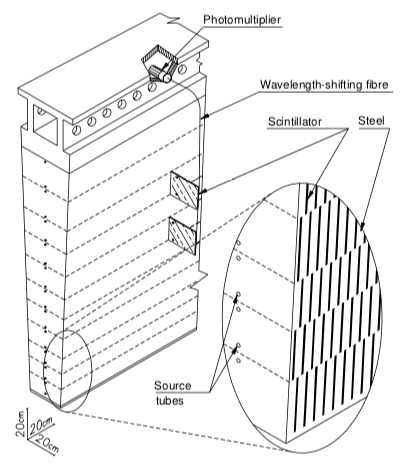
\includegraphics[width=0.4\textwidth]{figures/chapter2/calorimeters/atlas_tile_module}
        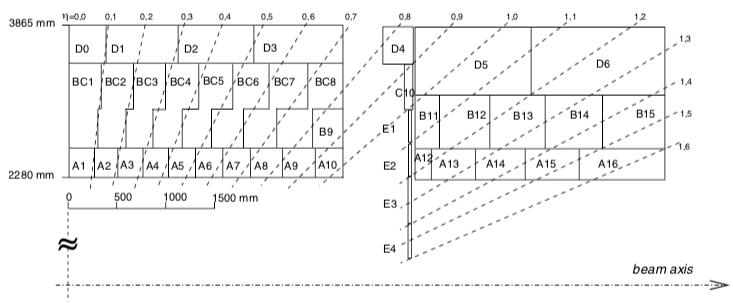
\includegraphics[width=0.9\textwidth]{figures/chapter2/calorimeters/atlas_tile_plan_view}
        \caption{
            Figures taken from Ref.~\cite{CERN-LHCC-96-042}.
            \textbf{\textit{Top}}: A view of a tile calorimeter module with its interleaved steel
                absorbers and scintillating tiles and PMT readout. Also indicated are the source tubes
                through which radioactive Cesium (Cs) sources are passed for calibration purposes~\cite{Marjanovic:2018ohl}.
            \textbf{\textit{Bottom}}: Illustration of the segmentation of the projective readout of
                both the barrel and extended barrel tile calorimeter.
        }
        \label{fig:tile_calo}
    \end{center}
\end{figure}

\FloatBarrier
\subsubsection{Forward Calorimeter}
\label{sec:calo_forward}

The forward calorimeter (FCal) system~\cite{Artamonov_2008} provides calorimetric coverage to
high $\lvert \eta \rvert$, between $3.1 < \lvert \eta \rvert < 4.9$,
furthering the hermeticity of the detector.
As indicated in Figure~\ref{fig:fcal}, FCal consists of three layers in the
$z$ direction: an electromagnetic layer (FCal 1) and two hadronic layers (FCal 2 and FCal 3).
All three layers use LAr as the active medium but differ in their passive media.
FCal 1 uses copper for its absorber, chosen for its heat removal properties,
while FCal 2 and FCal 3 use tungsten, chosen to provide high containment and
minimisation of the lateral spread of hadronic showers.
The FCal modules consist of matrices of the passive material with regularly
spaced readout tubes  oriented parallel to the beam-pipe that are filled with the cooled LAr.

\begin{figure}[!htb]
    \begin{center}
        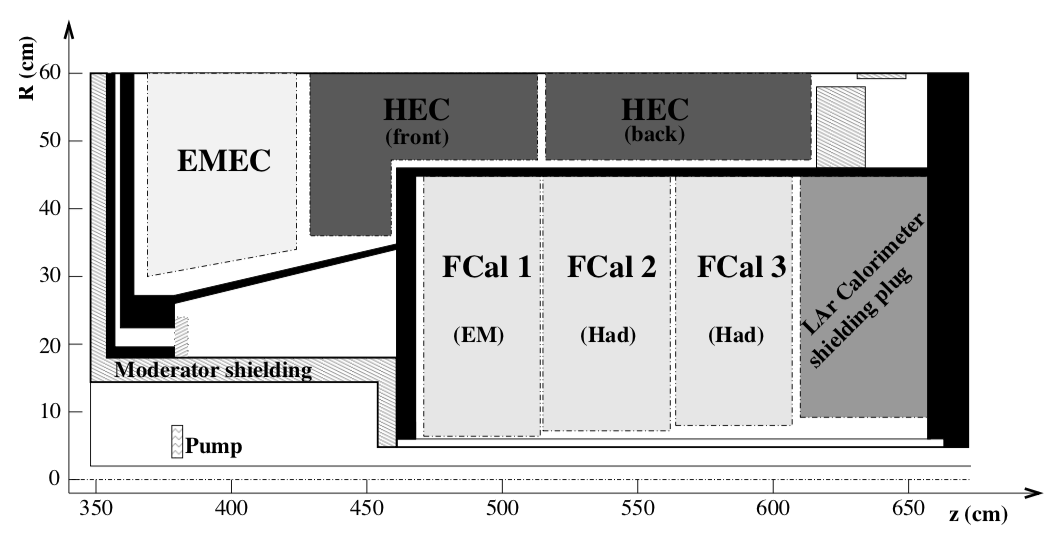
\includegraphics[width=0.65\textwidth]{figures/chapter2/calorimeters/atlas_fcal}
        \caption{
            View of the forward calorimeter (FCal) system. Portions of the electromagnetic
            and hadronic end-cap systems are also shown.
            Figure taken from Ref.~\cite{Artamonov_2008}.
        }
        \label{fig:fcal}
    \end{center}
\end{figure}


%%%%%%%%%%%%%%%%%%%%%%%%%%%%%%%%%%%%%%%%%%%%%%%%%%%%%%%%%%%%%%%%%%%%%
%%%%%%%%%%%%%%%%%%%%%%%%%%%%%%%%%%%%%%%%%%%%%%%%%%%%%%%%%%%%%%%%%%%%%
%
% MUON SPECTROMETER
%
%%%%%%%%%%%%%%%%%%%%%%%%%%%%%%%%%%%%%%%%%%%%%%%%%%%%%%%%%%%%%%%%%%%%%
%%%%%%%%%%%%%%%%%%%%%%%%%%%%%%%%%%%%%%%%%%%%%%%%%%%%%%%%%%%%%%%%%%%%%
\subsection{The Muon Spectrometer}
\label{sec:ms}

Surrounding the calorimeters is the muon spectrometer (MS)~\cite{CERN-LHCC-97-022}, responsible
for the detection of high-momentum, minimum-ionizing muons originating from the $pp$ interaction.
The MS is based on the magnetic deflection of muon tracks, allowing for their
momentum determination.
The bending of the muon trajectories is provided by the large
superconducting air-core toroid magnet system, illustrated in Figure~\ref{fig:atlas_magnet_system},
consisting of a large barrel toroid over the range $\lvert \eta \rvert < 1.4$
and end-cap toroid systems in the range $1.6 < \lvert \eta \rvert < 2.7$.
The superconducting toroid magnet provides an average field of $4\,$T.
The magnetic field bending strength is roughly constant in $\eta$, except in the
region in which the transition between the barrel and end-cap toroids takes place
($1.4 < \lvert \eta \rvert < 1.6$).
A view of the ATLAS detector is shown in Figure~\ref{fig:atlas_in_cavern},
where it can be seen that the volume enclosed by the MS takes up most of the available volume
outside of the calorimeter systems in the underground experimental cavern at Point 1.
It should be noted that the overall design of the superconducting toroid structure,
dictated by the performance requirements of the MS, is what gives ATLAS its large size and essentially
drove the original design of all subdetectors discussed in the previous sections.


\begin{figure}[!htb]
    \begin{center}
        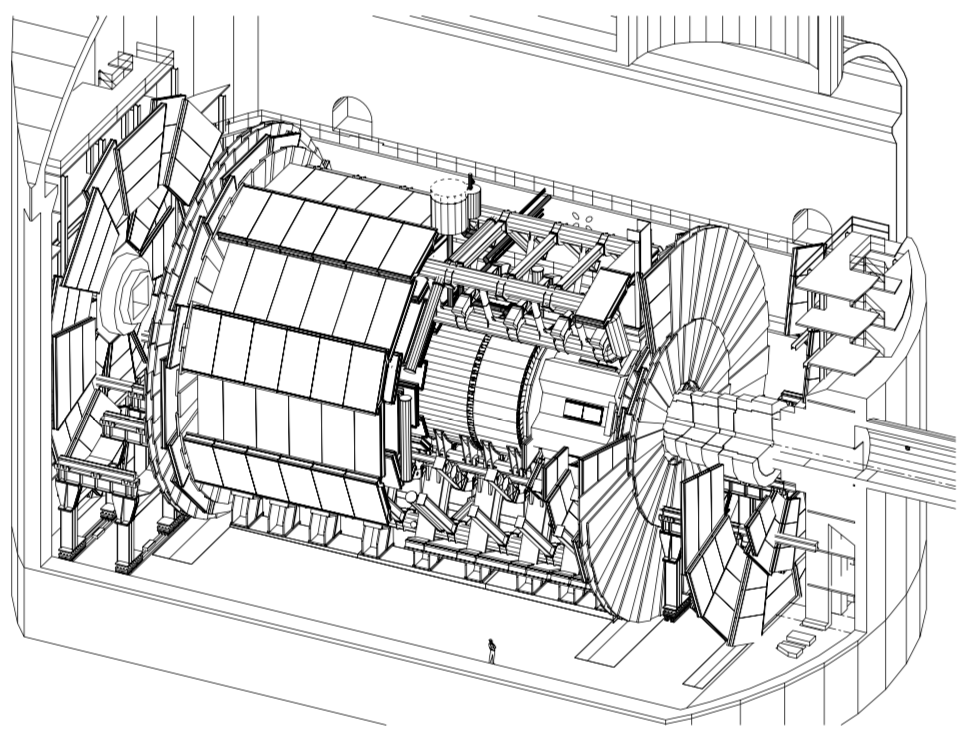
\includegraphics[width=0.8\textwidth]{figures/chapter2/atlas_in_cavern}
        \caption{
            A view of the ATLAS detector inside the underground experimental area
            UX15.
            The cut-away view exposes the toroid structure and
            calorimeter system.
            Notice that the outermost muon stations in the forward regions are located
            at the extreme ends of the cavern.
            Figure taken from Ref.~\cite{CERN-LHCC-97-022}.
        }
        \label{fig:atlas_in_cavern}
    \end{center}
\end{figure}
\FloatBarrier

There are four types of gaseous radiation detector used in the MS, and their chamber
layout is based on the concept of projective towers.
The chambers follow the structure of the toroid magnet structure and have a 16-fold segmentation
in azimuth, shown in Figure~\ref{fig:muon_segmentation}.
They are arranged in large and small sectors, with the large sectors covering
the regions between the coils of the toroid and the small sectors the azimuthal range
in which the coils sit.
The detector types can be broken into two classes and are either
\textit{precision} or \textit{trigger} chambers.
The precision chambers are composed of Monitored Drift Tube (MDT)~\cite{Bauer:2016gyg} and Cathode Strip Chamber (CSC)~\cite{Argyropoulos:2009zz}
detectors and allow for
the precise measurement the muon tracks as they traverse the MS, specifically the
precise measurement in the bending plane of these tracks so as to allow for accurate
determination of the muon momenta through their curvature.
The trigger chambers are composed of Resistive Plate Chamber (RPC)~\cite{Aielli:2006hg} and Thin Gap Chamber (TGC)~\cite{Majewski:1984ag}
detectors and have fast signal formation and readout times, allowing for
accurate assignment of a passing muon to a specific $pp$ bunch crossing.
Both types of detectors exist in the barrel and end-cap sections of the
MS and there are typically at least three layers of precision-type chambers over the
entire $\lvert \eta \rvert$ range of the MS in order to allow for the sagitta measurement
of the muon tracks necessary for momentum determination.
The number of precision chamber  hits over the entire range in $\eta-\phi$ of the MS
is shown on the left side of Figure~\ref{fig:muon_nchambers_crossed}. 
In the regions $\lvert \eta \rvert \sim 0$ and $\lvert \eta \rvert \sim 1.2$ there
are noticeable drops in chamber coverage in order to allow for ID and calorimeter
services and in the transition region between the barrel and end-cap, respectively,
as seen on the right side of Figure~\ref{fig:muon_nchambers_crossed}.


\begin{figure}[!htb]
    \begin{center}
        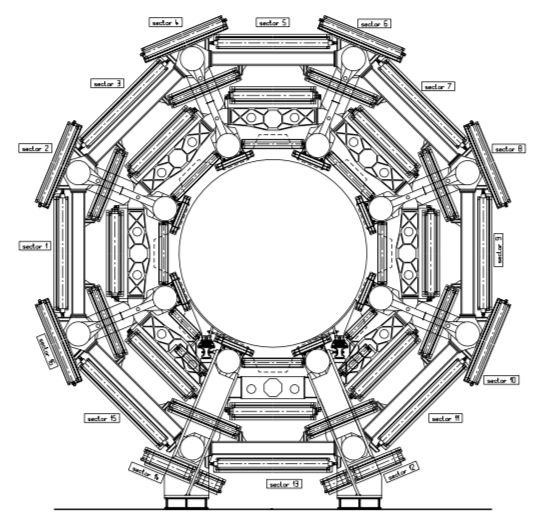
\includegraphics[width=0.4\textwidth]{figures/chapter2/muon_spec/atlas_muon_barrel}
        \raisebox{0.4cm}{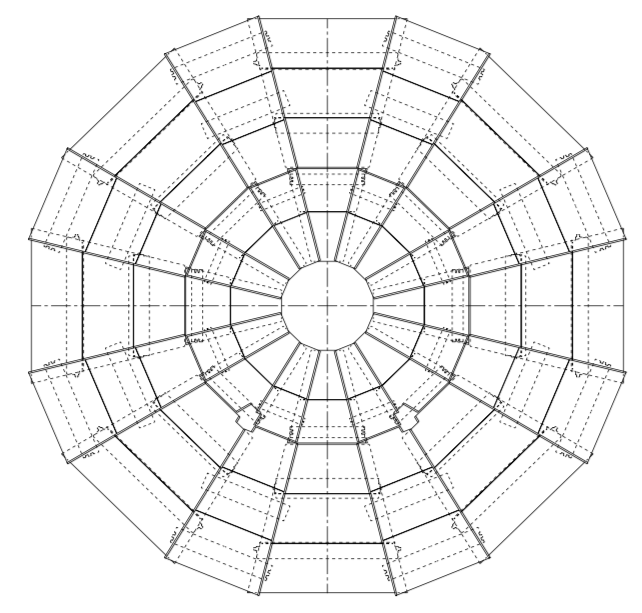
\includegraphics[width=0.35\textwidth]{figures/chapter2/muon_spec/atlas_muon_endcap}}
        \caption{
            View of the 16-fold segmentation of the muon spectrometer in the barrel (\textbf{\textit{left}})
            and end-cap (\textbf{\textit{right}}).
            Clearly seen in both is the arrangement of the detector chambers into large and
            small sectors, allowing for complete coverage in azimuth.
            The view of the end-cap is that only of the MDT chambers located at $z\approx13$\,m.
            Figures taken from Ref.~\cite{CERN-LHCC-97-022}.
        }
        \label{fig:muon_segmentation}
    \end{center}
\end{figure}

\begin{figure}[!htb]
    \begin{center}
        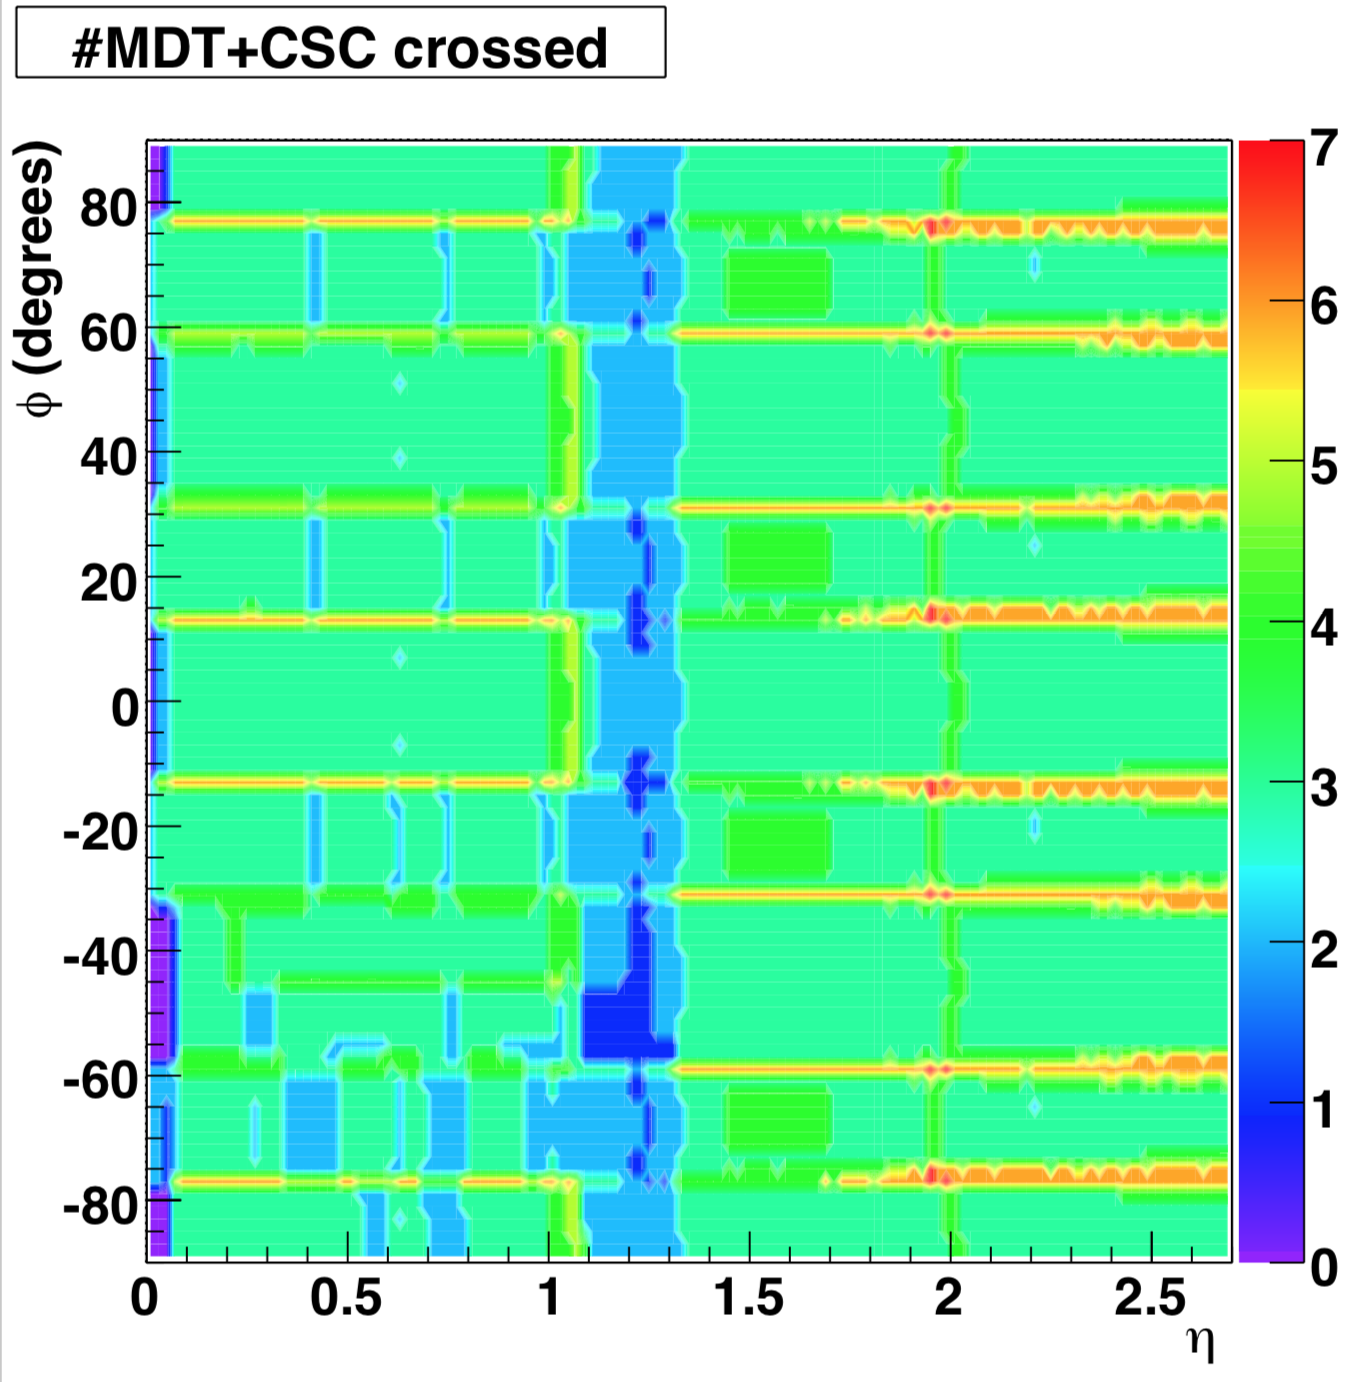
\includegraphics[width=0.4\textwidth]{figures/chapter2/muon_spec/atlas_ms_nchamber_crossed}
        \raisebox{0.6cm}{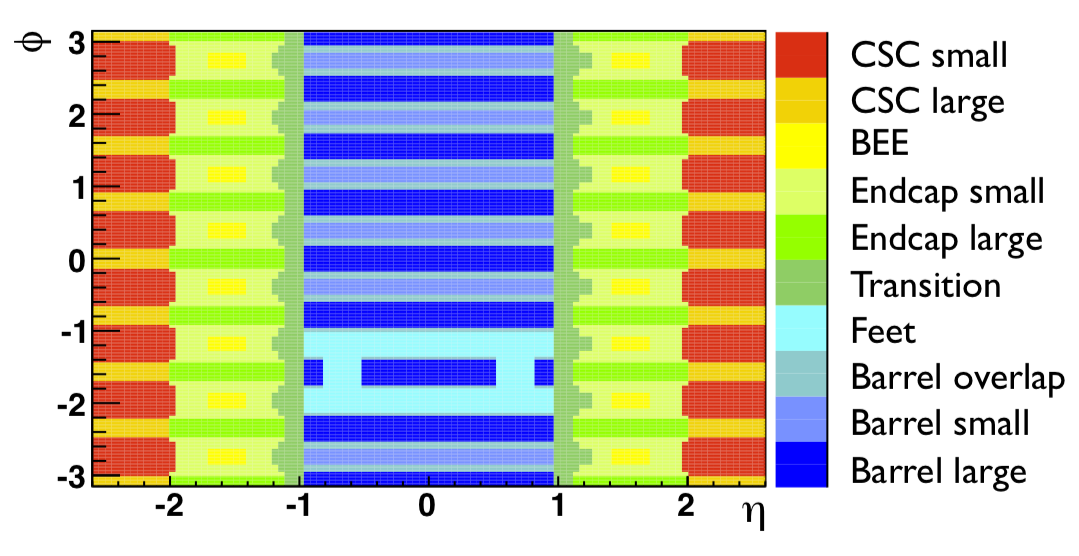
\includegraphics[width=0.58\textwidth]{figures/chapter2/muon_spec/atlas_muon_overlap}}
        \caption{
            \textbf{\textit{Left}}: Number of precision muon chambers (MDT and CSC) traversed by a muon passing through the muon
                spectrometer as a function of $\eta$ and $\phi$.
                The regions of high numbers of crossings ($>4$) correspond to the regions of overlap
                between the large and small sectors.
                Figure taken from Ref.~\cite{ATL-PHYS-PUB-2009-008}.
            \textbf{\textit{Right}}: Location in $\eta-\phi$ of several regions of the MS. Figure taken from Ref.~\cite{Mete:1454661}.
        }
        \label{fig:muon_nchambers_crossed}
    \end{center}
\end{figure}
\FloatBarrier

The layout of the muon chambers and the corresponding detector technologies
in the barrel and end-cap sections is shown in Figure~\ref{fig:muon_plan_view_eta}.
Here we will briefly describe each, starting with those in the barrel section.

\begin{figure}[!htb]
    \begin{center}
        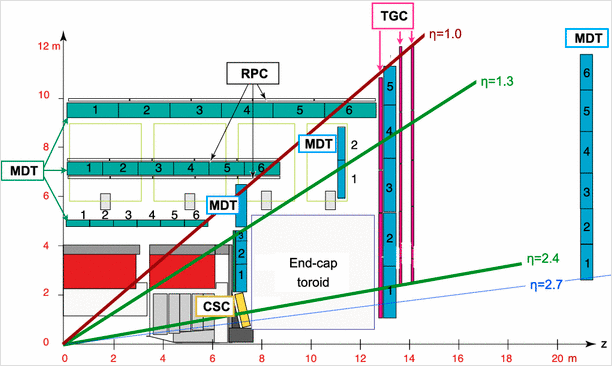
\includegraphics[width=0.8\textwidth]{figures/chapter2/muon_spec/atlas_muon_plan_view_eta}
        \caption{
            A view in the $r-z$ plane of a quadrant of the muon spectrometer (MS).
            Indicated by color are the four detector technologies used in the MS:
            MDT (blue), RPC (grey), TGC (red), and CSC (yellow).
            The light grey boxes at $6 < r < 9$\,m indicate the location of the
            barrel toroid structures.
            Also shown are the envelopes in $\lvert \eta \rvert$ of the barrel,
            small wheel, and big wheel sections of the MS.
            Figure taken from Ref.~\cite{MuonTrigPerf8}.
        }
        \label{fig:muon_plan_view_eta}
    \end{center}
\end{figure}
\FloatBarrier

\subsubsection{Muon Spectrometer: Barrel}
\label{sec:ms_barrel}

The muon chambers in the barrel section of the MS are rectangular in shape and arranged in 3 cylindrical shells,
concentric about and parallel to the beam-axis at radial distances of 5, 7.5, and 10.5\,m (see Figure~\ref{fig:muon_segmentation}).
The precision chambers in the barrel section are composed of MDT chambers
with tubes perpendicular to the beam-axis and parallel to the toroidal magnetic field,
allowing for precision measurement along $\eta$.
The MDT tubes are $3\,$cm in diameter and contain a 93\% Ar -- 7\% CO$_2$ gas mixture
with a single tungsten-rhenium wire operated at $3$\,kV.
Traversal of a minimum ionising particle (MIP) ionises the gas within the tube,
and the signal of the resulting ionisation charge is read out.
The typical spatial resolution of a single MDT tube is below $100\,\micron$.
The MDT chambers are built as multi-layers of many MDT tubes which allows for the improvement
of the spatial resolution down to $50\,\micron$ when the information from the individual layers is combined.
An MDT double multi-layer chamber is shown in Figure~\ref{fig:mdt_chamber}.
Also illustrated in this figure is the principle by which the tube hits in a given MDT
multi-layer are used to form tracklets which aid in the process of muon track-building.

\begin{figure}[!htb]
    \begin{center}
        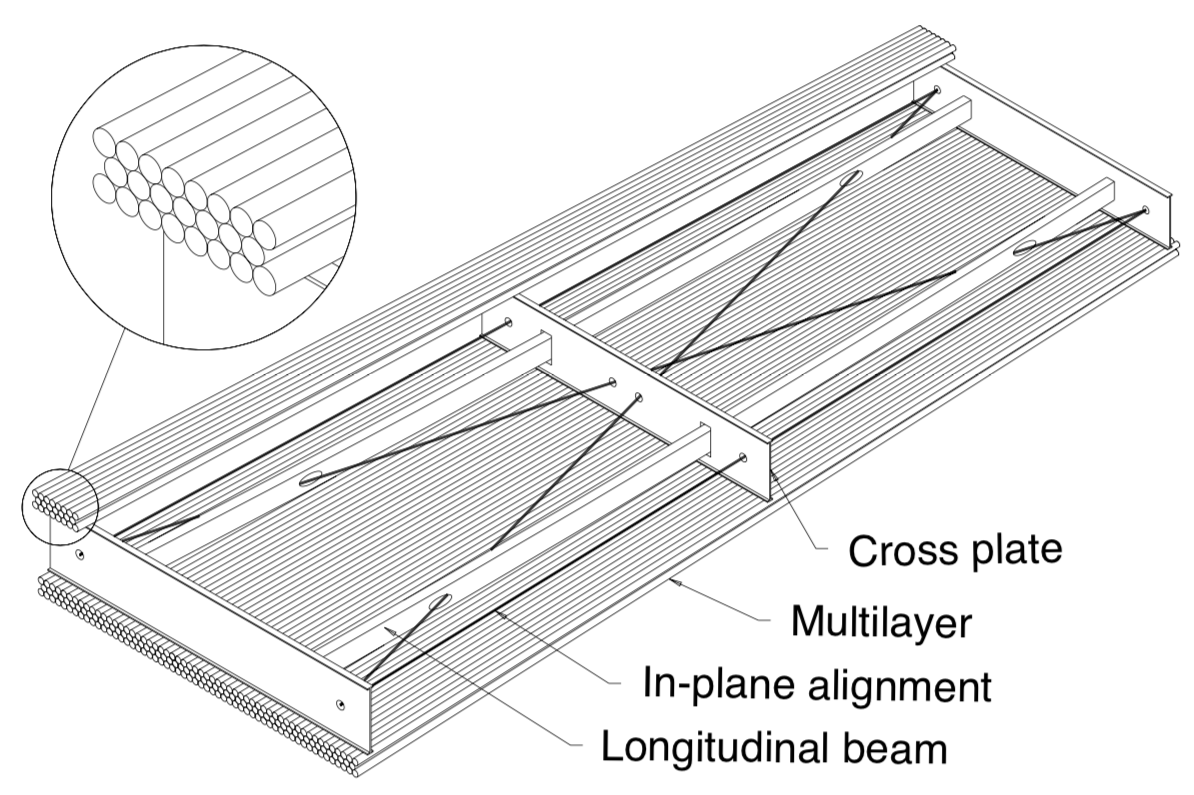
\includegraphics[width=0.5\textwidth]{figures/chapter2/muon_spec/mdt_chamber}
        \raisebox{1.22cm}{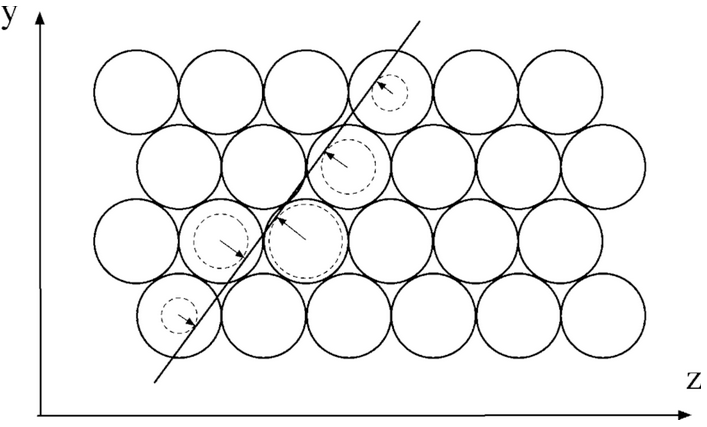
\includegraphics[width=0.32\textwidth]{figures/chapter2/muon_spec/mdt_trackfit}}
        \caption{
            \textbf{\textit{Left}}: Illustration of a double-multilayer MDT chamber with its internal alignment
                and support structure exposed. A zoom-in on the multilayer of MDT tubes is shown.
                Figure taken from Ref.~\cite{CERN-LHCC-97-022}.
            \textbf{\textit{Right}}: Illustration of the multilayer MDT tracklet-fitting algorithm~\cite{MDTtrackfit}.
        }
        \label{fig:mdt_chamber}
    \end{center}
\end{figure}

The chambers responsible for constructing muon trigger primitives in the MS barrel
are the RPC chambers, whose principle of operation is shown on the left of Figure~\ref{fig:muon_trigger_chamber}. 
The RPC gap is 2\,mm, filled with tetrafluorethane (C$_2$H$_2$F$_4$), and is lined with
parallel plate electrodes operated at a potential difference of 9.8\,kV. This high operating
potential and gas mixture allows for a timing resolution of 2\,ns. Readout strips in $x$ and $y$
collect the induced charge from the ionisation events within the gap and provide
additional spatial information for track and trigger-primitive building.

\subsubsection{Muon Spectrometer: End-cap}
\label{sec:ms_endcap}

The end-cap muon chambers, located in $1 < \lvert \eta \rvert < 2.7$, are arranged
in 4 rings --- \textit{wheels} ---  extending radially and concentric with the beam axis at $z \approx 7.5, 10, 14, 22$\,m
from the $pp$ interaction point.
The wheel at $z\approx 7.5$\,m, located on the IP-side of the end-cap toroid, is referred to as the `Small Wheel' and those at $z>10$\,m are
referred to as the `Big Wheels'.
That at $z\approx 10$\,m, situated above the end-cap toroid, is an intermediate muon station composed of MDT chambers and has generally lower coverage than the
Small and Big Wheels.

As in the barrel section, the primary precision measurement in the end-caps is provided
by MDT chambers which are located in all four wheels of the end-cap.
The MDT tubes are oriented azimuthally in order to obtain precision measurement in $\eta$.
At the region $2 < \lvert \eta \rvert < 2.7$, in the innermost muon station
in the end-cap that experiences the highest background rates,
the precision muon measurement is provided by the CSC chambers at low radii.
The CSC detectors are multi-wire proportional chambers, illustrated in Figure~\ref{fig:csc_chamber},
with cathode strips perpendicular to anode wires and operated with Ar/CO$_2$/CF$_4$ gas mixtures.
Passing MIPs result in ionisation events whose signals along the strips and wires are
subsequently readout.
As compared to the MDT chambers, the CSC detectors can resolve spatial information in both $\eta$ and $\phi$
and, due to their relatively high granularity readout structure, can sustain the higher
background rates experienced in this very forward region of the detector.
The CSC sectors are multi-layered (4-layers) and can achieve spatial hit resolutions on the order
of $60\,\micron$.

The trigger chambers in the end-cap are composed of the TGC detectors.
Like the CSC, the TGC is a multi-wire proportional chamber with a gas mixture
of CO$_2$ and $n$-pentane ($n$-C$_5$H$_{12}$).
An illustration of the operating principles of a TGC detector is shown in Figure~\ref{fig:muon_trigger_chamber}.
The graphite cathodes and wires, with $1.4$\,mm separation, are held at a potential
difference of $2.9$\,kV.
This high potential difference and anode/cathode geometry allows for signals to be readout
with a timing resolution of 4\,ns.
The signals from the drift electrons, collected along the wires, and the induced
charge on the strips located behind the G-10 layer are read out and provide
two-dimensional spatial information that can be used both in track and trigger-primitive building.


\begin{figure}[!htb]
    \begin{center}
        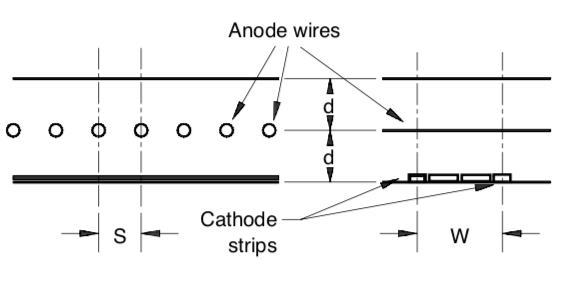
\includegraphics[width=0.55\textwidth]{figures/chapter2/muon_spec/csc_chamber}
        \caption{
            Diagram showing the main components of a cathode-strip chamber (CSC).
            On the \textbf{\textit{left}} (\textbf{\textit{right}}) is a view parallel (perpendicular) to the anode
            wires and perpendicular (parallel) to the cathode strips.
            Figure taken from Ref.~\cite{CERN-LHCC-97-022}.
        }
        \label{fig:csc_chamber}
    \end{center}
\end{figure}

\begin{figure}[!htb]
    \begin{center}
        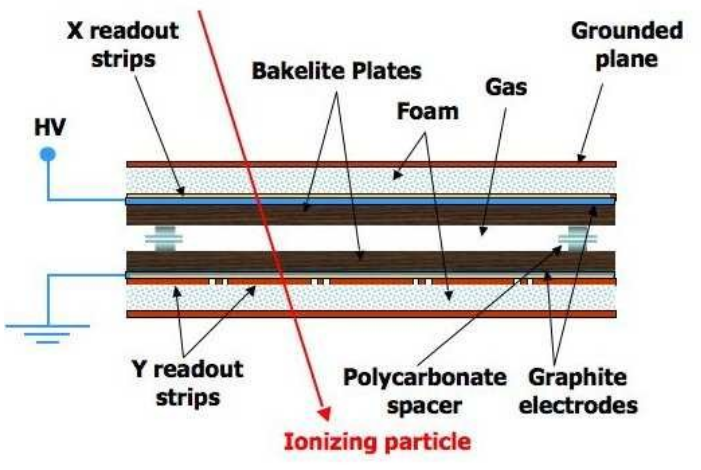
\includegraphics[width=0.5\textwidth]{figures/chapter2/muon_spec/rpc_chamber}
        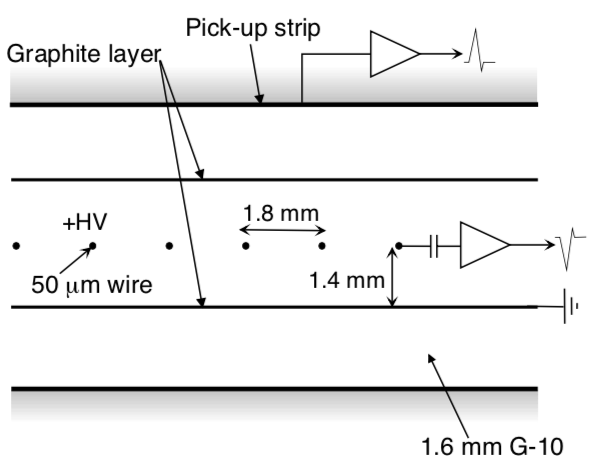
\includegraphics[width=0.38\textwidth]{figures/chapter2/muon_spec/tgc_chamber}
        \caption{
            Muon trigger chambers. Figures taken from Ref.~\cite{CERN-LHCC-97-022}.
            \textbf{\textit{Left}}: Illustration of a resistive plate chamber (RPC) and its principle of operation.
            \textbf{\textit{Right}}: Diagram showing the main components of a thin-gap chamber (TGC).
        }
        \label{fig:muon_trigger_chamber}
    \end{center}
\end{figure}


%%%%%%%%%%%%%%%%%%%%%%%%%%%%%%%%%%%%%%%%%%%%%%%%%%%%%%%%%%%%%%%%%%%%%
%%%%%%%%%%%%%%%%%%%%%%%%%%%%%%%%%%%%%%%%%%%%%%%%%%%%%%%%%%%%%%%%%%%%%
%
% TDAQ
%
%%%%%%%%%%%%%%%%%%%%%%%%%%%%%%%%%%%%%%%%%%%%%%%%%%%%%%%%%%%%%%%%%%%%%
%%%%%%%%%%%%%%%%%%%%%%%%%%%%%%%%%%%%%%%%%%%%%%%%%%%%%%%%%%%%%%%%%%%%%
\subsection{Trigger and Data Acquisition}
\label{sec:tdaq}

During Run 2 operation between 2015--2018, the LHC delivered $pp$ collisions to ATLAS at instantaneous luminosities of
$10^{34}$\,cm$^{-2}$s$^{-1}$, at a bunch spacing of 25\,ns, giving 33.7 $pp$ interactions per bunch crossing on average
(see Figure~\ref{fig:int_lumi_multiyear}).
These values correspond to roughly $10^9$ $pp$ interactions per second.
It is not possible for the ATLAS detector and data storage facilities to both respond to and record every one of these interactions.
In fact, from a physics perspective it is not necessarily desirable to record every single interaction.
The vast majority of such interactions arise from uninteresting, soft collision processes which are not likely
to contain, for example, decays of Higgs bosons or of new particles not accounted for in the SM.
For this reason, the ATLAS detector employs an \textit{online}\footnote{The `online' environment refers to that of the
ATLAS detector during runtime. The `offline' environment refers to anytime in which the data being inspected
or analysed is not \textit{at that time} being recorded by ATLAS but instead has already been stored to permanent storage
and is readily accessible at any time.}
selection strategy to select potentially interesting candidate events to be further processed and considered
for permanent storage. This online selection strategy is referred to as the \textit{trigger} system~\cite{Jenni:616089}.

The ATLAS Run 2 trigger system consists of two levels: a hardware-based low-level
trigger, referred to as the \textit{Level-1} (L1) trigger, and a second level software-based high-level trigger (HLT)~\cite{PanduroVazquez:2244345}.
The L1 trigger uses relatively coarse-grained measurements from the calorimeters and MS.
It performs the first level of selection, reducing the initial input 40\,MHz rate of events by
accepting events at a maximal rate of 100\,kHz.
The L1 trigger performs searches for coarse proxies of interesting physics objects: leptons, photons, and jets.
It triggers on electrons and photons based on energy deposits in the EM calorimeter, limited to $\lvert \eta \rvert < 2.5$.
The hadronic calorimeter provides jet candidates to the L1 trigger system via calorimeter `towers' made up of
trigger elements constructed by a sliding window algorithm.
Each trigger element is constructed by calculating energy sums of calorimeter cells in $\eta - \phi$.
Muon-based L1 triggers are based on coincidences of hits along the layers of the MS that form
projective towers, or \textit{roads}, consistent with high-\pT~muons.

The candidate events selected by the L1 trigger system are forwarded to the HLT.
The HLT system is composed of a Level 2 (L2) trigger and the event filter (EF).
The L2 system is similar to the L1 trigger, but performs more refined measurements on the objects and
regions of the detector that resulted in the initial L1 trigger's decision to accept the event.
The EF is purely software based, using the ATLAS Athena reconstruction framework~\cite{AthenaRef}
to perform high level object reconstruction and identification using algorithms similar to those used
in the offline environment and described in Chapter~\ref{chap:objects}.
The HLT accept rate is roughly 1\,kHz.
The accepted events are sent to CERN's permanent storage facilities and are made ready for the offline analysis.
An overview of the trigger system is shown in Figure~\ref{fig:run2_trigger}.


\begin{figure}[!htb]
    \begin{center}
        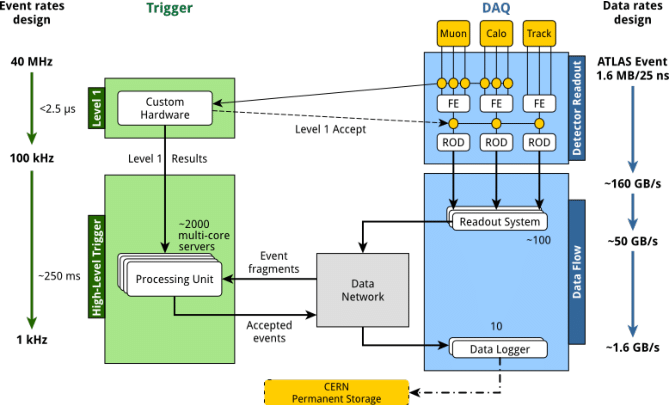
\includegraphics[width=0.7\textwidth]{figures/chapter2/tdaq/atlas_run2_trigger_system}
        \caption{
            Overview of the ATLAS Run 2 trigger and data-acquisition architecture.
            Data from the muon and calorimeter systems are used for the Level 1 (L1) trigger, reducing
            the input event rate from 40\,MHz to 100\,kHz.
            The data accepted by the L1 trigger are forwarded to the readout drivers (RODs)~\cite{Jenni:616089}
            which, among other things, re-shuffle the raw data into the standardized ATLAS event format~\cite{Bee:683741}.
            The events selected by the HLT at a rate of 1\,kHz are pulled from the RODs and then forwarded to the permanent
            storage.
            Figure taken from Ref.~\cite{PanduroVazquez:2244345}.
        }
        \label{fig:run2_trigger}
    \end{center}
\end{figure}

